%
% LaTeX report template 
%
\documentclass[a4paper,10pt]{article}
\usepackage[final]{graphicx}
\usepackage[english]{babel}
\usepackage[latin1]{inputenc}
\usepackage{comment}
\usepackage{subfigure}
\usepackage[section]{placeins}
\usepackage{float}
\usepackage[margin=1in]{geometry}
\usepackage{setspace}

\usepackage{hyperref}
\hypersetup{
    colorlinks=true,
    linkcolor=blue,
    filecolor=magenta,      
    urlcolor=cyan,
}


%
\begin{document}
%
   \title{Super Cherry Tomato Kartz Design Overview}

   \author{Joseph Miller 504744848, Jorge Hurtado 704595625 \\ Xilai Zhang 804796478, Patrick Chau 404793486}
          
   \date{}

   \maketitle
   
   \tableofcontents
 
  \newpage
   
\doublespacing

\section{Introduction}
This report provides an overview of our design for a local multiplayer kart racing game. We outline the requirements of the project as well as cover the motivations behind our design choices, and the techniques used to implement them. Additionally, we review complications faced over the quarter and explain how our project fits into a larger context. The requirements listed for our project were to incorporate the following: 

\singlespacing
\begin{itemize}
\item Speech Recognition
\item Localization
\item IMU Sensor Inputs
\item Communications
\end{itemize}

\doublespacing

\noindent
We designed a four player split racing game, providing a third person view for each player. Integrating speech recognition as the activating factor for the power-ups acquired during the race by players. While providing live video feed of the racer in first place during the race. Each kart is steered by controller tilt input from custom built controllers. 

For the purposes of developing the game, we split the duties into several subsystems: Application, Camera, Speech, and Hardware. The Hardware aspect involves a set of 4 controllers we designed that communicate with a Python server. This server filters the input messages before delivering them to the application in Unity. Unity manages running all of the game related content and relies on the system microphone to handle Speech Recognition and the python UDP camera stream. These duties are described in detail in the following sections.

\section{Basic Design}
\begin{figure}[H]
  \centering
      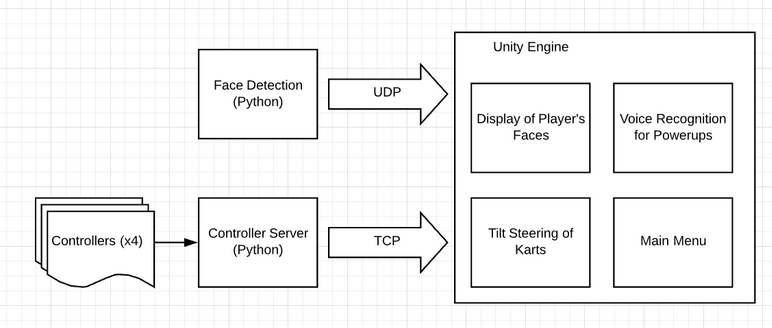
\includegraphics[width=0.95\textwidth]{Assets/System.png}
  \caption{System Overview of Super Cherry Tomato Kartz.}
\end{figure}


\section{UI and Preliminary Server Work (Xilai)}

\begin{figure}[H]
  \centering
      
\includegraphics[width=0.6\textwidth]{Assets/Unity.png}
  \caption{Unity Hub (left) and running Unity project (right).}
\end{figure}

Unity is a graphical interface that is capable of communicating with other electronics, i.e. internet of things. Unity Hub manages all unity projects and stores each project as a hierarchy tree on your local computer. A unity project displays content by continuously rendering frames and scenes. The initial scene in our project, for example, is the main menu.

 \begin{figure}[H]
  \centering
      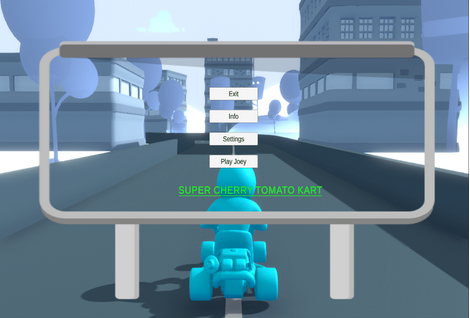
\includegraphics[width=0.6\textwidth]{Assets/MainMenu.png}
  \caption{Super Cherry Tomato Kartz Main Menu.}
\end{figure}

In our starting scene, we put a gigantic but invisible canvas object in front of our main camera. Having a canvas object is crucial because it allows us to add components on to it, such as a billboard. In this project, we set the billboard to the background and make it transparent, so that users can look through it and have a view of the racing environment. Upon starting the project, players can hear the sound of engines and background music. On the main menu, players can choose from four options: "play", "exit", "info" and "settings".  Players can click the "play" button to start the game, "info" button to read information about the game, "exit" to get out of the game. Clicking the play button, for example, takes us to the four player main game scene.

 \begin{figure}[H]
  \centering
      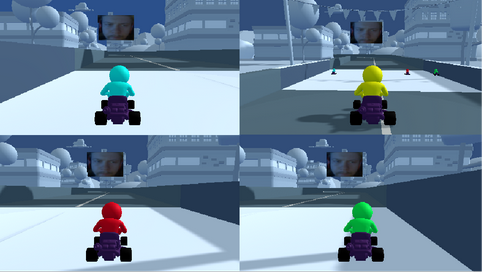
\includegraphics[width=0.6\textwidth]{Assets/MainGame.png}
  \caption{4 Player race scene that can be accessed from the main menu.}
\end{figure}

Clicking the info button gives the player an introduction to the game mechanics. As careful readers might have noticed, we applied a filter to the initial scene to create the visual effect of a "dreamy environment".

 \begin{figure}[H]
  \centering
      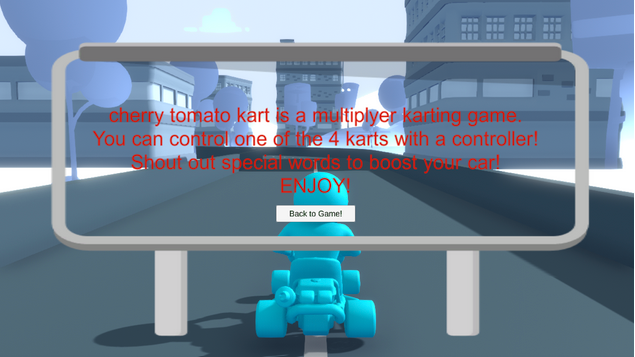
\includegraphics[width=0.6\textwidth]{Assets/Info.png}
  \caption{Info scene for the game. This section has a dreamy environment filter applied.}
\end{figure}

Under each of these submenus, we also provided a "back" button to take players back to where they were, in case the players changed their minds. Pressing the R key at any time will also restart the application and bring players back to the main menu scene.


\subsection{Navigation}
In unity, scenes are treated as assets and can call upon each other. However, triggering and rendering another scene creates overhead and causes delay. Thus to avoid such burden on the server, we use quick navigation when there is no significant amount of change in the view. More specifically, quick navigation is achieved by hiding 3D objects and revealing 3D objects. Take the main menu view for example, when we click the "play" button, we are not rendering a new scene at all. Instead, we hide our four buttons ( play, exit, settings, info) and instead reveal another two buttons which were previously invisible (play, back). 

 \begin{figure}[H]
  \centering
      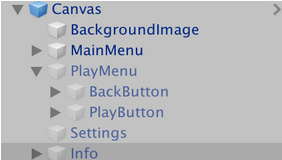
\includegraphics[width=0.6\textwidth]{Assets/InitialScenes.png}
  \caption{Initial state of the scenes.}
\end{figure}

Note that the main menu is active, visible, and highlighted in color blue, whereas other scenes such as the play menu are grayed out, and invisible in the initial scene. Upon clicking the buttons, we call upon the SetActive function attached to each element, and change the visibility of corresponding elements. 

 \begin{figure}[H]
  \centering
      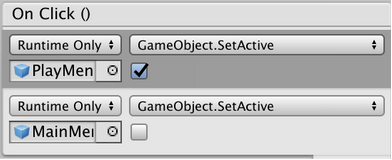
\includegraphics[width=0.6\textwidth]{Assets/OnClick.png}
  \caption{UI menu for setting assets as Active or Inactive.}
\end{figure}

Described above is a good way to navigate when changes are minor. But what if we have a lot of changes? In that case it is unrealistic to configure the visibility of all components because there are too many. Instead, we invoke scripts to render another scene for us. This can usually be achieved by calling upon the loadScene function. But in order to have a proper triggering, we need to attach the script to an object, triggering from a non object will fail (which took me a long time to debug). Finally, we would like to transfer our scenes from one unity project to another. To achieve a compatible merge of unity projects and keeping all the nice navigations, we concatenate scenes by creating packages and transferring the packages. 

 \begin{figure}[H]
  \centering
      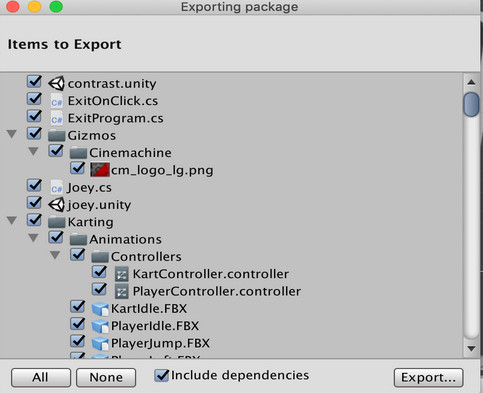
\includegraphics[width=0.5\textwidth]{Assets/Export.png}
  \caption{UI menu for setting up a package for export.}
\end{figure}

When creating and exporting packages, do remember to select those that are unique to the current scene and not duplicate and overwrite existing elements. Also remember to include dependencies. These steps of transferring scenes are important for integration between different unity projects.
Navigation also gives our project the strong ability to recover from failures. In case our system breaks down, we receive keyboard input, reset objects and navigate back to the initial scene. 
Moreover, the navigation techniques we have discussed in this section are unique to our project. Other groups render all components in a single scene and thus do not need navigation.


\subsection{Audio}
Based on feedback from midterm presentation, in this version of the game I added in cool audio effects. In the starting main menu scene we have authentic audio kindly provided by Joey, and also background music from the Mario Kart games. We switch music when loading different scenes to give players different sorts of enjoyment. 
 \begin{figure}[H]
  \centering
      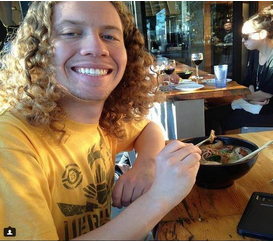
\includegraphics[width=0.3\textwidth]{Assets/Joey.png}
  \caption{Lead voice actor for the game: Joey.}
\end{figure}

\subsection{Primitive Server}
The primitive unity server has a direct connection via TCP sockets to raspberry pis, through C\# scripts. The connection was via eduroam instead of UCLA WIFI to resolve hostname issues. (Figured this out with the help from Pavan. Thanks!)
The primitive unity was later adapted to its current form because hostname could not be resolved on Joey's computer. And the solution to that was having the unity talk to the python server I wrote last quarter, and from the python server we connect to the raspberry pis. 
The primitive unity was the first version that successfully established connection to raspberry pis in our session, with proper multi threading and buffering


\section{Controllers, Server, and Unity (Joey)}
My responsibilities included working on the controller and hardware aspects related to the project, designing the server client architecture for the game, and performing Unity programming related to implementing Power Ups and player controls for the main game. These are all outlined in their own respective sections.
 
\subsection{Hardware}
The game controller is itself made out of hardware and should ideally be soldered to a perf board, but it can also be assembled on a breadboard. The following parts list and wiring diagram explains how the system can be built in the event that one wishes to use one. In terms of circuit design, There are four capacitive debouncing circuits to allow for smooth voltage transitions on the button presses preventing multiple inputs from a single press. Finally there is an LED connected directly to a GPIO pin to a current limiting resistor and ground. This LED is a network status LED that will notify the user if the controller has connected with the server or not. It will be in one of two states: the first is blinking signaling that it is attempting communication and the second is solid indicating it has connected successfully to the server.

\subsubsection{Parts List}
The following list and circuit schematic be used to purchase and assemble one's own controllers.

\singlespacing
\begin{itemize}
\item 4 x Raspberry Pi Zero W
\item 16 x 1$\mu$F capacitors
\item 16 x Push Buttons
\item 4 Ideally different colored LED
\item 4 x 1k$\Omega$ Resistors and 16 x 10k$\Omega$ Resistors
\item 4 x BerryIMU sensor
\end{itemize}
\doublespacing

\subsubsection{Circuit Schematic}

\begin{figure}[H]
  \centering
      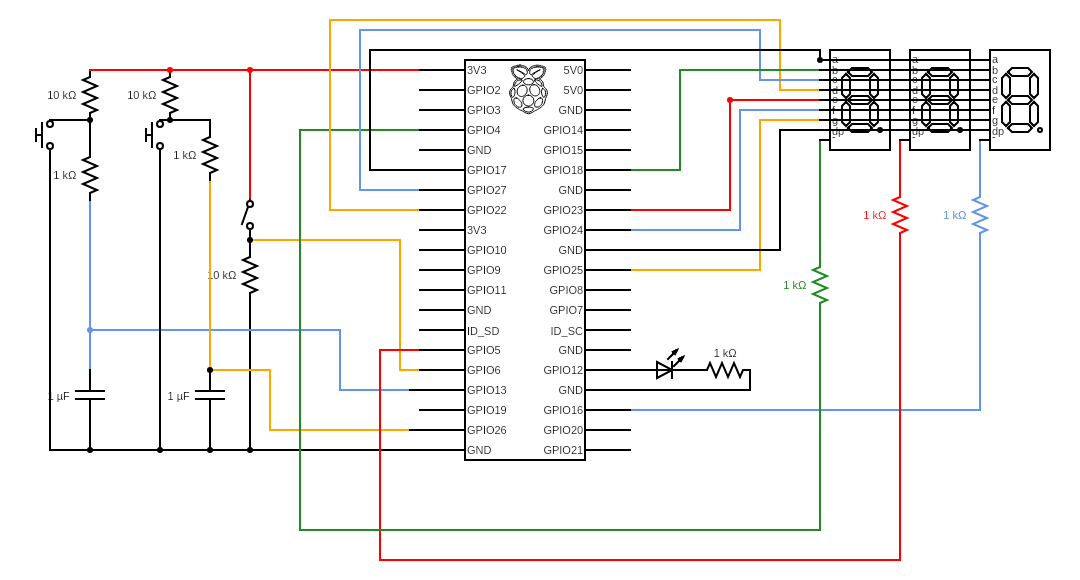
\includegraphics[width=0.95\textwidth]{Assets/circuit.png}
  \caption{Circuit schematic used for wiring the hardware token.}
\end{figure}

\subsection{Converting Hardware Token to Controller}
The hardware token was written in C and has it's own makefile to allow for ease in compilation. It was previously made up of a total of 8 files in addition to the makefile: hardware.c, hardware.h, globals.h, hardware\textunderscore token.c, network.c, network.h, signal\textunderscore handler.c, and signal\textunderscore handler.h. The header files contain function declarations and global variables. All function declarations are commented to show what inputs/outputs are involved in the function as well as what the function is supposed to do. These design ideas were maintained in for the modifications needed to convert this into a usable controller. For a more detailed analysis of the hardware token and its design please refer to the report from last quarter. Two new files were created to support the IMU and a variety of files required changes to enable support for the controller itself. These include hardware.c, hardware.h, hardware\textunderscore token.c, globals.h, network.c and the newly created motion\textunderscore detector.c and motion\textunderscore detector.h. As seen with the hardware token, All POSIX complient function calls that are made have proper error handling associated with them to ensure that the proper error code corresponding to errorno is printed to STDERR along with a message describing what went wrong. 

\begin{figure}[H]
  \centering
      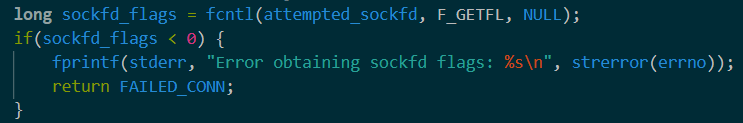
\includegraphics[width=\textwidth]{Assets/fcntl.png}
  \caption{Code showing error handling on POSIX function calls.}
\end{figure}

\subsubsection{Hardware Token File Change Log}
Additional constants have been added globals.h to accomodate the new buttons and jump signal. An additional pthread is generated in hardware \textunderscore token.c to accommodate the IMU thread. 

Hardware.c is the most modified file for this controller. All of the 7-segment code has been removed and all the GPIO pins have been remapped. Now there are 4 input GPIO pins to be read corresponding to the Up, Down, Drift and Item buttons. These pins are read on a 1ms interval with Mutexes to protect against contention on these shared variables. The LED is mapped to an output GPIO that exists in one of two states. If the server is connected, the LED is set to on and remains that way until the server is disconnected. When this happens, The LED GPIO is toggled on and off in 1 second intervals to indicate the server is trying to connect. All of the code pertaining to the 7 segment displays has become useless and exists merely as legacy code. 

The network thread in network.c has been modified to handle sending messages out at timed intervals. Now instead of waiting for a particular signal to be delivered to the network thread to indicate that a connection message should be delivered, a formatted string utilizing the global variables corresponding to button inputs is delivered to the Python server. These messages are sent as a series of 1's and 0's seperated by dots to indicate Up, Down, Left, Right, Drift and Item (e.g. 1.0.1.0.1.1 Means go up, left drift and use item). These strings are sent every 20 ms to give time for the Python server to receive, parse, and transfer the data to the main game server. Mutexes are used to prevent contention on shared variables across threads.

\subsubsection{Motion Detector.c and .h}
These files alongside the BerryIMU backend files are included in the controller design to map the Left and Right controller signals. The check scripts for the IMU in the BerryIMU backend all defaulted to exiting the program on receipt of an error. To make the program as robust as possible I added code to check for these conditions and loops with error messages to prevent the program from exiting prematurely and to alert the user to what happened with the controller's IMU. Inside the actual detector itself, the gyroscope sensor is utilized to read the x, y and z rotation angles, amplify them by a constant gain factor, convert them to degrees and finally be filtered through a complimentary filter that takes into account the current acceleration. These steps smooth out the signal from the gyroscope and allow for accurate angles over extended playtime. This allows a simple threshold detection method to be sufficient to determine left and right. Changes of 30 degrees from level is enough to determine left and right and the assignment of these is done under a mutex to prevent contention on these shared variables.

\subsection{Server client Architecture}
The server client architecture for the system involves the four controllers communicating with a central Python server that also servers as a client to the Unity Application. Communications between the controllers and Python is done over WiFi utilizing TCP and the Python server communicates with C\# over TCP through the computers localhost. Each of the controllers begin communication with the server by sending their MAC address. This allows the Python server to track each of the individual players based on their MAC Addresses. If a player disconnects and reconnects it will be reassigned to the same player it was originally associated to. The formatted strings sent from the controller that were described in the Hardware Token changelog are parsed in this Python server and aggregated. The Python server has 20 milliseconds to read input from all 4 controllers and format a new string associating the controlls for that given frame to each of the players in the game. This is then delivered to C\# over TCP for a minimal latency of 40ms from button press. This amounts to at minimum only a couple frames of latency between button presses. In practice the latency is hardly noticeable from a gameplay perspective and the controls feel butter smooth.

\begin{figure}[H]
  \centering
      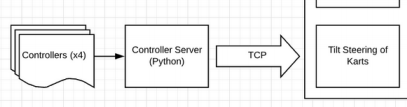
\includegraphics[width=0.6\textwidth]{Assets/TCP.png}
  \caption{Diagram showing Server Client Relationship.}
\end{figure}

On the C\# server end, public static strings are used to store the received strings from the Python server and are utilized in the "KeyboardInput.cs" script to control the player. In this script, each of the individual inputs are checked based on the ID of the object calling the script to determine whether to accelerate forward or backward, turn left or right, drift or use an item. Each input string is formatted with a unique player tag followed by the inputs pressed. Each of the unique player instructions are loaded into the public static string corresponding to the player number (e.g. P1:0.0.1.0.1.1P2:0.0.0.0.0.1 would have 0.0.1.0.1.1 stored in the string for player 1 and 0.0.0.0.0.1 stored in string for player 2).

\subsection{Unity Design}
Unity is the game engine we utilized to design the game itself. My main contributions for Unity involved getting power ups to work, get the players to be controlled by the controllers and create a scene hierarchy that allows the Server, Facial Recognition and Speech Recognition scripts to always be loaded and never destroyed.
\subsubsection{Power Ups}
The game utilizes Power Ups in a unique way compared to most off the shelf products. Typically in games such as Mario Kart or Crash Team Racing, Power Ups are obtained and delivered at random via power up boxes on the stage. We remove the random element these games have and allow the players voice to determine the power up they can use. On the controller is a dedicated power up button that can be pressed to activate a power up given two conditions are met: 1. The player has obtained a power up 2. The speech detection has detected that one of the 5 power up names have been said.


Power up boxes are managed by the Item Box manager and its attached ItemBox.cs script. This manager checks a global static string that will be in one of three states: used, noone, and the player name. When a player collides with the box, their object ID is stored as the value for the power up status string and all other power up boxes are made inactive by the manager. In the KeyBoardInputs.cs script, powerups are then assigned to the player whose name matches the ID for this public static string before setting it to the noone state. Finally once a powerup is activated by the player, this string is updated to the used state and the powerUp manager reactivates the item boxes.


When a player is set to having a power up, the particle manager object attached to them is set to the play status to allow it to start spawning purple particles. This gives a visual indication that a player has a power up they can use. Once they use the power up, the particle manager is set to the pause state and the particles seize to spawn.
\begin{figure}[H]
  \centering
      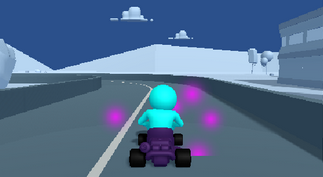
\includegraphics[width=0.5\textwidth]{Assets/Particles.png}
  \caption{Player with particles coming off them indicating they can use a power up.}
\end{figure}

There are five useable power ups in the game that are activated by running unity co-routines. Quick spawns a co-routine that multiplies the current players velocity and acceleration by a factor of 5 for 1 second giving them a major speed boost. Stop multiplies the velocity and acceleration by 0 to immediately stop them in their tracks. The idea behind this one is that it can be used by the other players who don't have the power up to rob the player with it of their advantage. By yelling stop as the player calls out their power up and pushes the button to activate it could cause stop to trigger over what they attempted to use. Paint is a power up that blocks all other players screens to disorient them for 5 seconds. This is a achieved by setting all other player's camera's field of view to 0 temporarily. Shrink is a power up that multiplies the player models x, y, and z scale by 0.25 causing them to be tiny. They also have their max speed capped to 90\% the usual max for a short while. This power up affects all but the person who used it. Finally invincible gives the player who uses it immunity from negative power ups for the remainder of the game. When checking for who to apply things like stop or shrink to, the game will also check if the player has invincibility or not. 

\begin{figure}[H]
  \centering
      
\includegraphics[width=0.5\textwidth]{Assets/Paint.png}
  \caption{Player having activated paint. All screens but the player who activated it are temporarily blocked.}
\end{figure}

\subsubsection{Scene Design}
There are 4 players and 4 cameras that are used for the main game scene. This inclusion of 4 cameras allows for a 4 player splitscreen experience as all of the cameras are attached to the respective player and have their screen coordinates mapped to one of 4 quadrants on the screen.

There is a scene that is always loaded that simply contains the billboard used to display the faces and the scripts for the server, speech detection and face detection scripts. These objects attached to this always loaded scene are marked with the DontDestroyOnLoad() function that prevents the object the scripts are attached to from ever being unloaded from the game world.

\section{Speech Detection (Jorge)}
Developing our speech recognition program there were a couple things I had to keep in mind in order to ensure that the program I developed was implantable into our game. First, was response time. In order for this to work effectively as a power up activation, computations had to be close to real time to provide a fluid experience to the user. Furthermore, I had to take into account the detection sensitivity of the program. As more than likely this game would lead to creating a loud environment, sensitivity would be very important in order to properly distinguish between background noise and intended input. 
 
Our speech recognition program originally relied on C\# library called System.Speech. This version response time was superb during standalone development; however faced issues disassociating background noise resulting in more than optimal false readings. Before managing to solve these issues, I discovered that it failed to integrate smoothly into Unity. 
 
As a result, I developed a second speech recognizing program that utilized a native Unity Speech Library in order to speed up access time. The final program used begins listening upon initiation, updating each frame. It listens for power up phrases listed in a keyword array. Upon a successful match a switch statement handles what occurs in game depending on the power up called. In the second version of this program confidence constraints were made to be easily changed by the developer in order to allow ourselves to better tune the sensitivity levels. Additionally, I included a print out of time stamps for every successful listen as well as the confidence percentage which sped up testing significantly the second time around. 

\section{Facial Detection (Patrick)}
The goal for the face detection was to display the face of the player in first place. This script was built using OpenCV's library, taking inspiration from their face detection example. The script saves the file locally and sends a message over a UDP socket to the Unity engine to then update the image in the game. 


How the facial detection works is that it uses a Haar cascade classifier trained with positive and negative images of faces. Due to time constraints and lack of data, I used a pre-trained classifier provided in the OpenCV examples. The theory behind this is that there are around 100,000 features used in this classifier, each feature being a Haar-like feature. This refers to a . Together, each feature makes this a strong classifier but it would be very long to compute every feature for every frame. What makes this a cascade classifier is that instead of computing all the features at once, they are broken up into stages with the strongest features being checked earlier on. Only if a frame passes all stages is it detected as a positive. This speeds up computation time by a decent amount. One downfall however is that it has a rather high false positive rate. The script then scans over the image at varying rectangle sizes and records any positive matches that it finds in the form of 2 (x,y) points making up a rectangle.
\begin{figure}[H]
  \centering
      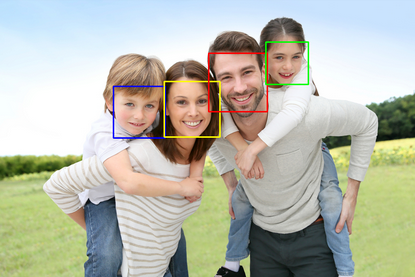
\includegraphics[width=0.4\textwidth]{Assets/FacialRecognition.png}
  \caption{Stock photo showing bounding boxes for faces from OpenCV.}
\end{figure}


What I found though is that the script detects faces in no particular order. To maintain the association of a face to a player, the faces, once localized, need to be tracked. This is done by first computing the centroids of each face. The face is saved as 4 points making up a rectangle so this is simple enough. The centroid is computed for all new locations and all old locations. We then compute the distance from each old face to each new face. Locations are then then updated a saved face location with the newer location with the least distance from the old location. This works under the premise that people don't move that quickly, especially with an update time of around 5ms. However, we must also ensure uniqueness to avoid all face regions so there is a check to make sure that a new update location is not already chosen by another old face. In the event that two update locations chose the same old face, the tiebreaker is done by choosing the smaller distance of the two.


Once the list of faces is finalized, the new list of bounding boxes for each face is saved for the next iteration. A message is sent over UDP to the Unity server for it to then read the image in and render it on the billboard. Additionally, Unity will also indicate which player is in first place and then send the position to the Python script so it knows which player's face to save on its next cycle. UDP was chosen to reduce latency as much as possible. TCP is inherently slower than UDP for two reasons: it's a connection-oriented protocol and it has error correction and acknowledgement packets. These two slow down the process significantly compared to UDP which has neither. 


The game, upon startup, will start the process automatically by invoking a call to the Process library. This was done with the intention to maximize portability for working across computers and environments. This necessitates that the user's Python library folder path is entered into "PlayerControllerScript.cs" and that the user's Python environment has numpy and opencv-python both installed. It will then periodically check the UDP buffer to see if there is an update message. If so, it will look in the saved image and pull it and re-render the texture in the game. This occurs every cycle such that it gives the impression of video, although at a very low frame rate. There was no significant impact on gameplay by having this although it could be done more efficiently but having some form of lock-out method. This would improve it because, oftentimes, the client will try to pull the image after receiving the update but the script has not yet finished writing and will throw an exception. So the efficiency of this operation could be improved in that way.

\begin{figure}[H]
  \centering
      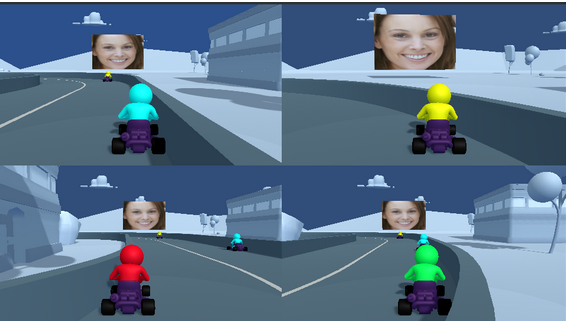
\includegraphics[width=0.4\textwidth]{Assets/Face.png}
  \caption{Yellow player is in first place so the face with yellow bounding box is displayed on the billboard.}
\end{figure}

\section{Encountered Issues and Workarounds}
Throughout the project there were a number of snags we hit for which workarounds needed to be instated. These issues took up a good portion of time that could have been spent implementing additional features to the game. It is a part of the design process and we managed to meet the original goals set up for the project despite these issues setting us back.

\subsection{Hardware Failures}
Right towards the end of the project was when the hardware we had began to suddenly give up on life. Two Raspberry Pi Zero W's had their Micro-SD cards suddenly die resulting in a significant time sync to obtain and flash new cards to get the Pi's up and running again. Furthermore, the soldering on the perf board ate up a huge amount of development time due to a significant amount of hardware debugging and issues with button press detection. It seems as if the boards purchased didn't properly map some GPIO pins requiring major soldering, desoldering and per controller code modification. Finally two of the BerryIMU devices were damaged. One only lost its magnetometer which thankfully was not relevant to this project. The other lost its gyroscope, accelerometer and magnetometer leaving it completely useless. These issues resulted in a demo only being available showcasing three controllers as new parts could not be ordered and delivered in the time we were given between hardware failure and demo.

\subsection{Facial Detection}
Our original approach to localizing the players was to have all the controllers have a colored LED on them. The camera would detect this patch of color and then find the closest face found to that patch. This way, the players would be able to be detected. However, what I found was that the color detection ranges are very hard to get right, and are not robust given the variability of settings players could be in. The workaround here was to have the players sit in a predetermined order when the game starts up. This was from left to right from the point of view of the camera, with player 1 on the left and player 2 on the right. After this point, the players' faces were then tracked as described before.

\subsection{Speech Detection}
Unfortunately, while the original speech recognition program developed worked flawlessly I found several issues when importing the script into unity. It seems that there were issues with Unity calling functions from the System.Speech library. After several attempts to facilitate seemingless access to Unity, the best version still resulted in an unbearable amount of latency. Ultimately, I had to redevelop the program so that it would rely on a Unity based speech library. By doing so it vastly improved the response time such that we could implement it as a tool in the game.

\subsection{End Scene}
Another issue we ran into was finalizing our end scene. While I (Jorge) was able to build the general format and aesthetics of this transition, we were unable to fully integrate this into our game. Unfortunately, when transitioning scenes we lost vital player information in regards to placement when trying to display it on screen. In hindsight, I believe this issue arose from the lack of continuous overarching scene that could hold this information during transition. I think Joey faced a similar issue when integrating the video component to the game; however, due to the lack of time towards the end of quarter we were unable to test this theory.

\section{Future Plans}
Super Cherry Tomato Kart has a myriad of advancements that can be made. Ideally if this were planned for a widespread audience there is a lot more work to be done to bring this up to the standards seen in the indie gaming community. 

\subsection{3D Printed Case}
A 3D printed case will allow for improved ergonomics and control for users playing the game. It also allows all the internals to be hidden away from the user and provides padding in case the device is dropped during gameplay. Furthermore, it provides a more aesthetically pleasing design giving it a much more professional look and feel.

\subsection{PCB}
\begin{figure}[H]
  \centering
      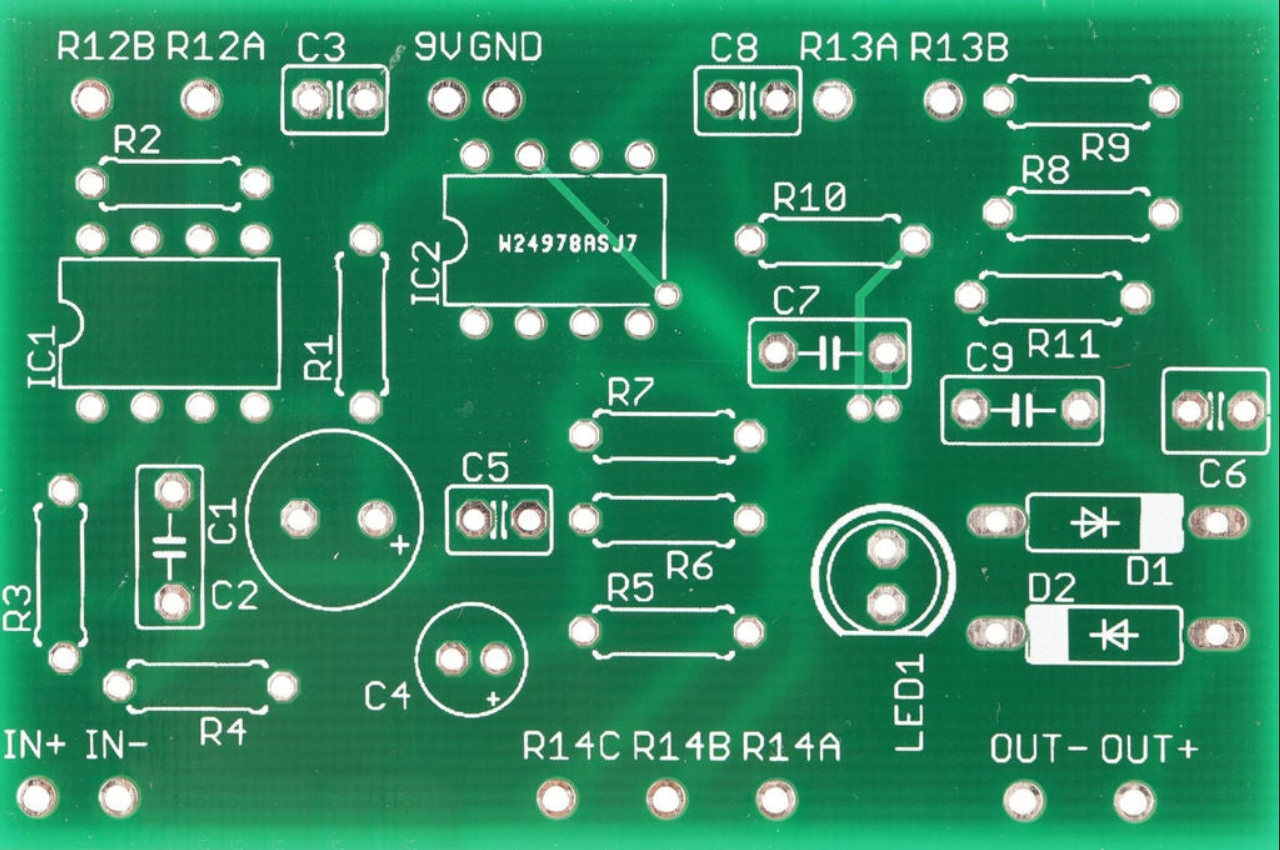
\includegraphics[width=0.5\textwidth]{Assets/PCB.png}
  \caption{Sample printed circuit board that shows how easily components could be soldered together without worrying about cutting and soldering connecting wires.}
\end{figure}

Having a printed circuit board for soldering the components for the controller will significantly reduce the difficulty in connecting all of the components together and allow for a more compact design. This will make development of a 3D printed controller case easier and allow for case designs to be more compact as well.

\subsection{More Levels}
Currently the game features a simple racetrack with no complicated twists and turns. To become a more fun and versatile racing game, more complicated tracks could be designed with obstacles that move around the track that slow players down. Furthermore, speed pads could be implemented to give players temporary speed boosts upon contact. The ideas are limitless and would increase the fun and replay ability potential of the game and thus its possibility for commercial success. 

\subsection{Option for Number of Players}
As the game currently stands, it only supports a fixed number of players: 4. It would be ideal to allow groups of 1, 2 or 3 to play the game as well against an AI or AI's. This would be a major undertaking as it would require designing strong and weak virtual opponents, but would be a necessity for this to ever be viable in the indie racing game market. Adding this option to the main menu and modifying the camera positions would be relatively straightforward to add given a short amount of time.

\subsection{Additional PowerUps}
Since PowerUps are activated via voice, addition of new ones is limited only by how distinct the words are from each other and how likely the speech detection is capable of picking them up. Once adequate names are decided upon and tested, unique powerUps such as Reverse or Grow could be constructed in the playerControl script. The idea behind reverse would be all other player controls would be inverted so up is down and left is right. This causes the players to temporarily lose some control of the vehicle and gives the original player an edge. The idea behind grow would be the opposite of shrink. The player who uses it will grow big and move faster than their opponents for a short while.

\section{Experimental Verification}

Overall experimental verification was done primarily during standalone phases of our subsections. Each section was expected to meet its respective requirements before integration in efforts to streamline integration. We opted for an incremental integration approach to ensure respective components functioned properly before complicating the overall system. Unfortunately, due to this approach we were unaware of some issues until later in the quarter.

\subsection{Speech}
When testing our speech recognition component of this project, we had to keep multiple factors in mind. Most important was overall functionality as we envisioned creating a fluid audio component for our users. This breaks down into multiple sub standards that must be met. First, was response time. In order for this to work effectively as a powerup activation, computations had to be performed close to real time. We measured this by comparing timestamps of successful hearings and comparing them to our projected speech time. By doing so we had a better idea of the actual response time of our program. Additionally, I had to take into account the detection sensitivity of the program. As more than likely this game would be played in a loud environment, sensitivity would be very important in order to properly distinguish between background noise and intended input. In order to better test our programs sensitivity, I made sure we could not only see the confidence readings of each word heard. Additionally, it can be easily modified by the developers to better fit the current environment the system is used in.

\subsection{Facial Detection}
When testing the camera system, there were two main components which needed to work: communicating with the server and finding the correct image. Communication with the server was deemed to be functional if the message both arrived correctly to the Unity client with low latency following a new player achieving first place. In initial testing, the system correctly found the player in first place and did send the message to the Python script, but there was a huge delay between a sent message and a read message. What happened here was that with the UDP connection, the buffer would fill with garbage and not be cleared on a read. This was easily remedied by decreasing the amount of empty messages being sent and once this was done, the latency was almost non-existent. Secondly was finding the correct image. Once the script received the player number, it would save the corresponding face. Once we swapped to the left-to-right player initialization and implemented the face tracking, this was a lot simpler. Faces were saved to a local directory that would modularly find the absolute path to increase portability of the program as a whole. This was then tested by running the python script and having it save the image. Again, there needed to be some handshake between the Unity client and the Python script for determining when to update the image because otherwise there would be serious latency issues. We tested each player moving into first place and watching the screen to see if it was properly updated to the correct face. Once it did so consistently, it was deemed a working module. With these two finished, the subsystem could be integrated into the project.

\section{Conclusion}
Overall the project was a major success and we managed to complete and integrate all parts of our project together. Utilizing our GitHub repository which can be found at \href{https://github.com/patrickchau/EE180DB-Project}{https://github.com/patrickchau/EE180DB-Project} we were able to work on each of our own sections and merge them together with minimal effort. Using version control and constant communication between the team allowed us to constantly make progress and take ownership over specific parts of the project. We each added our own unique flare and ideas to the parts of the project we had control over and worked together excellently to form a strong team. While there were a few things we didn't quite have the time to completely finish such as the Endgame scene, the resulting product is fun, easy to set up and easy to modify and build upon. 


\section{References}
[1] "Raspberry Pi GPIO Pinout," Raspberry Pi GPIO Pinout. [Online]. Available: https://pinout.xyz/. 

\noindent
[2] Technologies, Unity. "Unity User Manual (2019.3)." Unity, [Online] Available: 

\noindent
docs.unity3d.com/Manual/index.html. 

\noindent
[3]  Ozzmaker, BerryIMU, (2019), GitHub repository, [Online] Available: https://github.com/ozzmaker/BerryIMU

\noindent
[4] A. Greensted, "The Lab Book Pages," Sitewide RSS. [Online]. Available:

\noindent
http://www.labbookpages.co.uk/electronics/debounce.html

\noindent
[5] N3K EN, "Multiplayer Checkers Tutorial 6 - Server - Unity 3D[Tutorial]," Youtube Video. [Online]. Available: https://www.youtube.com/watch?v=3vFhnwgfP3U 

\noindent
[6] T. Daniels, "Speech recognition, speech to text, text to speech, and speech synthesis:" [Online] Available:

\noindent
https://www.codeproject.com/Articles/483347/Speech-recognition-speech-to-text-text-to-speech-a 

\noindent
[7] Docs.opencv.org. 2020. Opencv: Cascade Classifier. [online] Available at: 

\noindent
<https://docs.opencv.org/3.4/db/d28/tutorial\textunderscore cascade\textunderscore classifier.html> [Accessed 20 February 2020].

\noindent
[8] LightBuzz, Speech Recognition, (2017) GitHub repository, [Online] Available: 

\noindent
https://github.com/LightBuzz/Speech-Recognition-Unity

\noindent
[9] Docs.opencv.org. 2020. Opencv: Changing Colorspaces. [online] Available at:

\noindent
 <https://docs.opencv.org/trunk/df/d9d/tutorial\textunderscore py\textunderscore colorspaces.html> [Accessed 20 February 2020].
\end{document}
